\documentclass[margin=10pt]{standalone}
\usepackage{color,xcolor}
\usepackage{makecell}
\usepackage{tikz-qtree, tikz}
\usepackage{pgfplots}
\pgfplotsset{compat=1.11}
\usepackage[utf8]{inputenc}

\definecolor{myblue}{HTML}{0072BD}
\definecolor{mygreen}{HTML}{258F1B}
\definecolor{myred}{HTML}{C4000C}

\newcommand{\Ms}{\ensuremath{M_\mathrm{s}}} % Martensite start Temperature
\newcommand{\Mf}{\ensuremath{M_\mathrm{f}}} % Martensite finish Temperature
\newcommand{\As}{\ensuremath{A_\mathrm{s}}} % Austenite start Temperature
\newcommand{\Af}{\ensuremath{A_\mathrm{f}}} % Austenite finish Temperature

\usetikzlibrary{decorations.pathreplacing,arrows,shapes,positioning,shadows,calc}
\usetikzlibrary{decorations, decorations.text,backgrounds}
\tikzset{every picture/.style={font issue=\footnotesize},
    font issue/.style={execute at begin picture={#1\selectfont}}
}

\begin{document}
\begin{tikzpicture}
% [every node/.style={inner sep=0,outer sep=60}]
    \node[anchor=south west] (dsc) at (0,0) {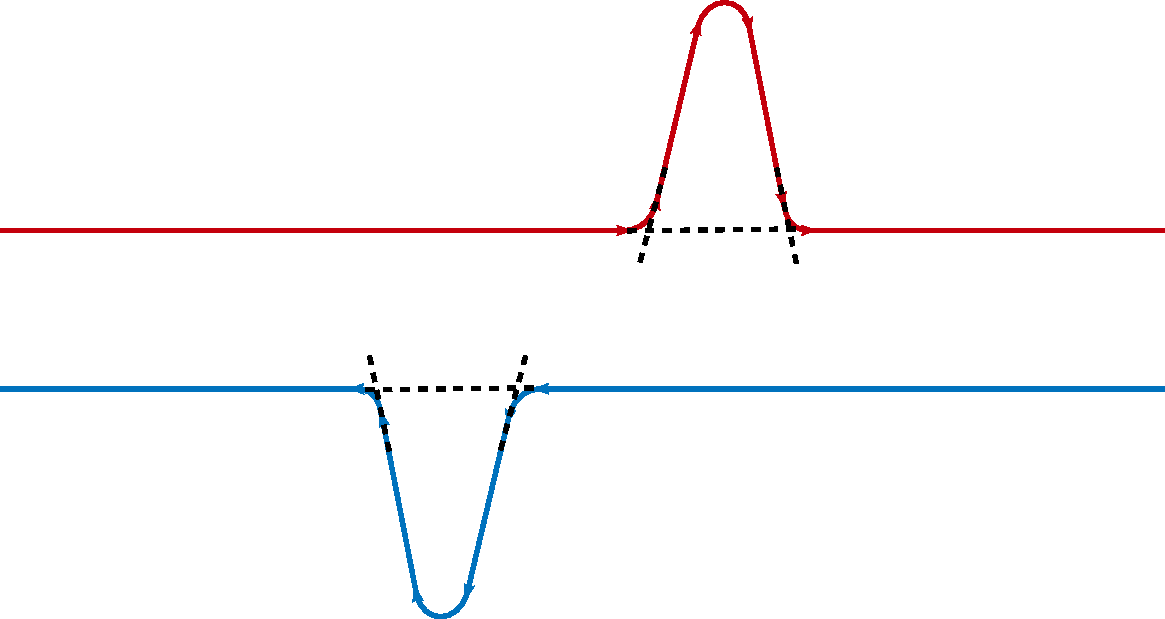
\includegraphics{dsc-curve.pdf}};
    \begin{scope}[x={(dsc.south east)},y={(dsc.north west)}]
        \draw[->,thick] (-0.11,-0.1)--(1.2,-0.1) node[pos=0.5,below,outer sep=10]{\textbf{\huge Temperature [$^\circ$C]}};
        \draw[->,thick] (-0.1,-0.11)--(-0.1,1.2) node[pos=0.5,above,sloped,outer sep=10]{\textbf{\huge Heat Flow [W]}};
        \node [anchor=center] (hheating) at (0.66,0.74) {\large $\Delta L_\mathrm{MA}$};
        \node [anchor=center] (hcooling) at (0.34,0.26) {\large $\Delta L_\mathrm{AM}$};

        \node [anchor=center] (MA) at (0.67,1.03) {\large $M\rightarrow A$};
        \node [anchor=center] (AM) at (0.33,-0.03) {\large $M\leftarrow A$};

        \node [anchor=center] (mf) at (0.22,0.41) {\large \Mf};
        \node [anchor=center] (ms) at (0.47,0.41) {\large \Ms};

        \node [anchor=center] (af) at (0.78,0.59) {\large \Af};
        \node [anchor=center] (as) at (0.535,0.59) {\large \As};

        % \draw[help lines, color=black, dotted] (-0.1,-0.1) grid (1.18,1.18);
        % \draw[black,ultra thick,rounded corners] (0.62,0.65) rectangle (0.78,0.75);
        \draw[help lines, color=black, dotted,xstep=.1,ystep=.1] (-0.1,-0.1) grid (1.18,1.18);
        % \foreach \x in {0,1,...,9} { \node [anchor=north] at (\x/10,0) {0.\x}; }
        % \foreach \y in {0,1,...,9} { \node [anchor=east] at (0,\y/10) {0.\y}; }
    \end{scope}


    % \node[anchor=center,yshift=40] (Atext)[below = of A] {\Huge Austenite};
    % \node[anchor=center,yshift=50] (twMtext)[below = of twM] {\Huge\makecell[c]{Twinned\\Martensite}};
    % \node[anchor=center,yshift=50] (detMtext)[below = of detwM] {\Huge\makecell[c]{Detwinned\\Martensite}};
    %
    % \path [-latex,ultra thick,bend left,color=mygreen] (twM.north) edge node [xshift=-20,pos=0.4,above,outer sep=10,color=mygreen] {\Huge$\sigma\uparrow$} (detwM.west);
    % \draw [-latex,ultra thick,color=mygreen] ($(detwM.east)+(0,0.5)$) arc(-90:180:3cm) node [xshift=30,pos=0.3,above,outer sep=10,color=mygreen] {\Huge$\sigma\downarrow$};
    % \path [-latex,ultra thick, bend left,color=myred] (detwM.east) edge node [xshift=25,pos=0.6,above,outer sep=10,color=myred] {\Huge$T\uparrow$} (A.north);
    % \draw [-latex,ultra thick,color=myblue] (A.west) -- node [midway,above,outer sep=10,color=myblue] {\Huge$T\downarrow$} (twM.east);

    % \path [-latex,ultra thick,out=135,in=225] (twM.north) edge (detwM.west);
    % \draw [-latex,ultra thick,out=0,in=90] ($(detwM.east)+(0,0.5)$) to [out=0,in=-90] ($(detwM.east)+(2,4)$) to [out=90, in=90 ] (detwM.north);
    % \path [-latex,ultra thick,out=0,in=90,looseness=3] ($(detwM.east)+(0,0.5)$) edge (detwM.north);
\end{tikzpicture}
\end{document}
